%pdflatex --shell-escape scap_benchmark_dl_training.tex

\PassOptionsToPackage{hyphens}{url}
\documentclass[compress,aspectratio=169]{beamer}

\usepackage[official]{eurosym}
\usepackage{multirow}
\setlength{\marginparwidth}{2cm}
\usepackage{todonotes}
\presetkeys{todonotes}{inline}{}
\usepackage[style=verbose,backend=biber,style=authortitle]{biblatex}
\setbeamertemplate{bibliography item}{\insertbiblabel} % Ensure that cite labels appear in references section
\addbibresource{ref.bib}
\usepackage{../assets/beamerthemeGoettingen} % make sure the theme file is on this path
\graphicspath{{../}{../assets/}}
\usepackage{caption}
\usepackage{booktabs}

\hypersetup{
    colorlinks,
    citecolor=black,
}

\newcommand{\source}[1]{\par\begin{textblock*}{6cm}(1cm,8cm)
    \begin{beamercolorbox}[wd=\paperwidth,ht=0.5cm,right]{framesource}
        \usebeamerfont{framesource}\usebeamercolor[fg]{framesource} \centering\tiny {#1}
    \end{beamercolorbox}
\end{textblock*}}


% listing / code
\usepackage{minted}
\usemintedstyle{tango}
% Box listing / code
\usepackage{tcolorbox}

% Box listing / code style 
% These options will be applied to all `tcolorboxes`
\tcbset{%
    noparskip,
    colback=gray!5, %background color of the box
    colframe=gray!20, %color of frame and title background
    coltext=black, %color of body text
    coltitle=black, %color of title text 
    fonttitle=\tiny,
    alerted/.style={coltitle=red, 
                     colframe=gray!40},
    example/.style={coltitle=black, 
                     colframe=green!20,             
                     colback=green!5},
    }

\lstset{literate=%
    {Ö}{{\"O}}1
    {Ä}{{\"A}}1
    {Ü}{{\"U}}1
    {ß}{{\ss}}1
    {ü}{{\"u}}1
    {ä}{{\"a}}1
    {ö}{{\"o}}1
    {~}{{\textasciitilde}}1
}

\usepackage{csquotes} % For \enqoute{}
\usepackage{hyperref}

% --- document configuration ---
\newcommand{\mytitle}{Benchmarking tree species classification\\with synthetic data and deep learning}     
% Leave empty for no subtitle
\newcommand{\mysubtitle}{My Subtitle}   
\newcommand{\myauthor}{Hauke Kirchner}
\newcommand{\myauthorurl}{\href{http://www.overleaf.com}{Something 
Linky}}
\newcommand{\myvenue}{Göttingen}
% For example, use \today
\newcommand{\mydate}{24.11.2022}
% For example, Institute for Computer Science / GWDG
\newcommand{\myinstitute}{GWDG - AG Computing}
% Leave empty for no footer image
\newcommand{\myfooterimage}{}           
\newcommand{\mygrouplogo}{}
% Images must be enabled manually under title page \titleLogo
% Adjust position and width manually for fewer images
\newcommand{\mytitleimageone}{}         
\newcommand{\mytitleimagetwo}{}        
\newcommand{\mytitleimagethree}{}

% --- title page ---
\title{\Large \mytitle}
\venue{\myvenue}
\date{\mydate}
%\subtitle{\mysubtitle}
%\authorURL{\myauthorurl}
\author{{\myauthor}}
\authorFooter{\myauthor \hspace{0.3cm} \includegraphics[height=1em]{\myfooterimage}}
\institute{\myinstitute}
\groupLogo{\includegraphics[width=2cm]{\mygrouplogo}}
\titleLogo{
%\includegraphics[height=2.7cm]{\mytitleimageone}
%\includegraphics[height=2.7cm]{\mytitleimagetwo}
%\includegraphics[height=2.7cm]{\mytitleimagethree}
}

\setbeamertemplate{footline}[text line]{
\begin{beamercolorbox}[sep=0.5em,wd=\paperwidth,leftskip=0.2cm,rightskip=0.1cm]{footlinecolor}
\myauthor \hfill \insertVenue \hfill \insertframenumber\,/\,\ref{pg:lastpage}
\end{beamercolorbox}
}

\begin{document}

\begin{frame}[plain]
	\titlepage
\end{frame}

\begin{frame}[t]{Table of contents}
  \tableofcontents[subsectionstyle=hide/hide]
\end{frame}

% --- slides begin ---

\section{Motivation}

\begin{frame}{Why is it important to benchmark the training process of neural networks?}

    \begin{columns}
        \begin{column}{0.5\textwidth}
            \begin{block}{\centering Training speed}
                \centering
                \vspace{3em}
                
\includegraphics[width=0.3\textwidth]{assets/speed_FILL0_wght400_GRAD0_opsz48.png}
            \end{block}
        \end{column}
        \begin{column}{0.5\textwidth}
            \begin{block}{\centering Energy efficiency}
                \centering
                \vspace{3em}
                
\includegraphics[width=0.3\textwidth]{assets/electric_bolt_FILL0_wght400_GRAD0_opsz48}
            \end{block}
        \end{column}
    \end{columns}

\end{frame}

\begin{frame}{Training speed 
              \begin{tabular}{@{}c@{}}
                  
\includegraphics[width=0.05\textwidth]{assets/speed_FILL0_wght400_GRAD0_opsz48.png}
              \end{tabular}
              }

    \begin{columns}
        \begin{column}{0.4\textwidth}
            \begin{itemize}
                \item training of neural networks is computational intensive
                \item $\Rightarrow$ workflow needs to be optimized for available hardware
                    \begin{itemize}
                        \item How many GPUs are worth to request?
                        \item What is the best set of software? (pytorch, cuda, ...)
                    \end{itemize}
                \item $\Rightarrow$ high impact of deep learning applications on energy consumption
            \end{itemize}
        \end{column}
        \begin{column}{0.6\textwidth}
            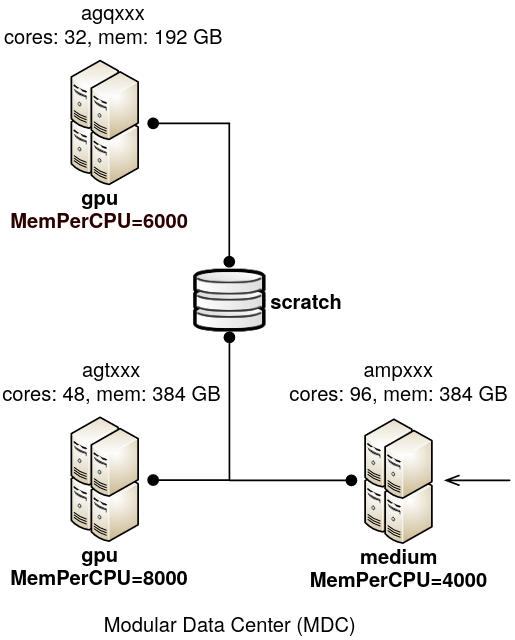
\includegraphics[width=1.1\textwidth]{assets/gwdg_scc.png}\\
        \end{column}
    \end{columns}

    \vspace{1.5 em}

    $\Rightarrow$ without optimisation for available accelerators future developments on ML/ deep learning will not be possible

    \source{Image source: \url{https://www.gwdg.de/web/guest/hpc-on-campus/scc}, Accessed on: 09.11.2022}
\end{frame}

\begin{frame}{Energy efficiency 
              \begin{tabular}{@{}c@{}}
                  
\includegraphics[width=0.05\textwidth]{assets/electric_bolt_FILL0_wght400_GRAD0_opsz48}
              \end{tabular}
              }



    \begin{columns}
        
        \begin{column}{0.6\textwidth}
            \begin{itemize}
                \item asdfasdf
            \end{itemize}


            $\Rightarrow$ as deep learning is emerging in several fields the impact on energy consumption and consequently our climate optimized training processes are essential
        \end{column}

        \begin{column}{0.4\textwidth}
            \vspace{-3.5em}
            \centering
            \begin{figure}
            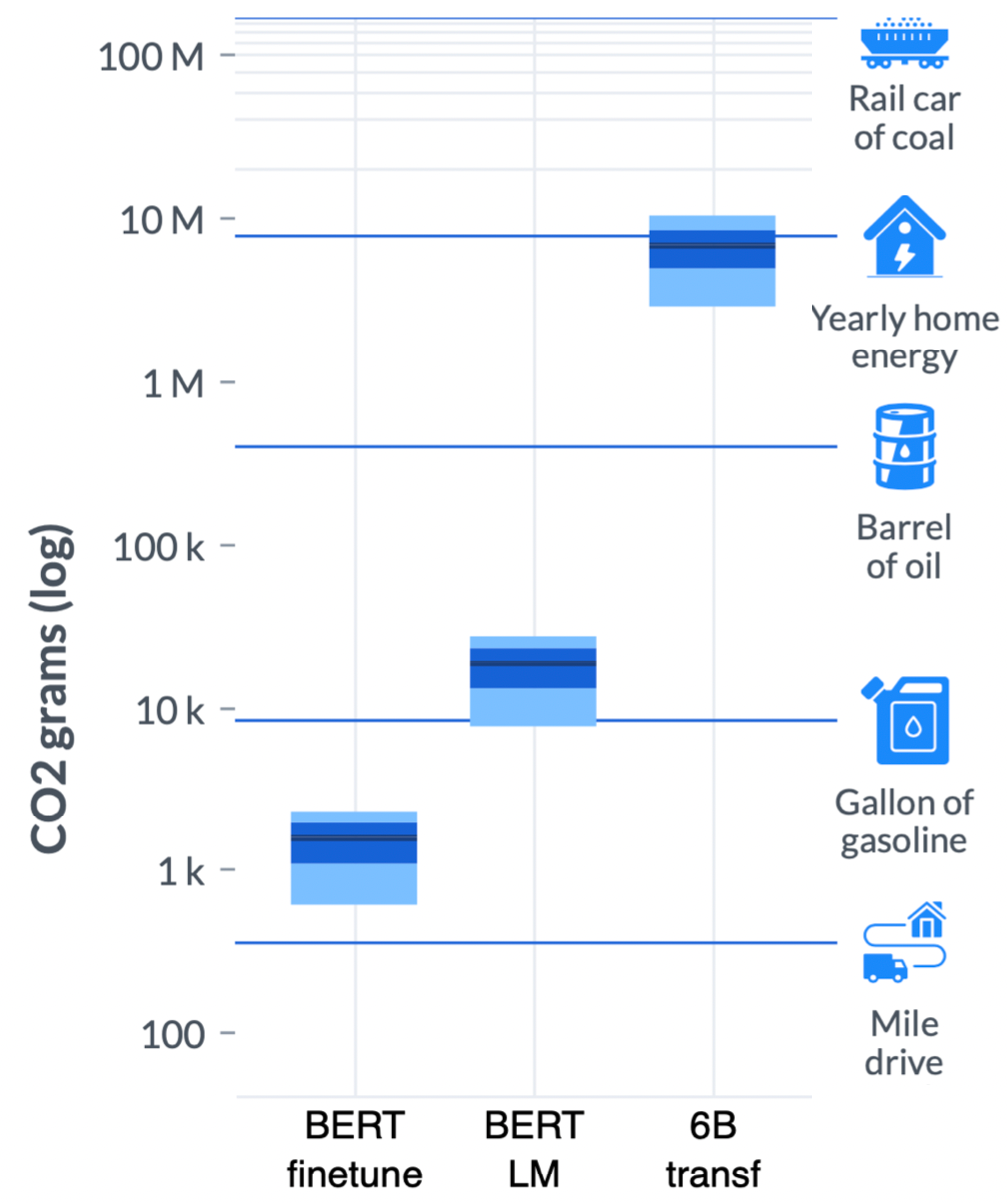
\includegraphics[width=\textwidth]{assets/20220610_dodge_measuring-the-carbon-intensity-of-ai-in-cloud-instances-fig2-bert.png}
            \caption*{$CO_2$ Relative Size Comparison}
            \end{figure}
            \source{Image source: Adapted from todo}
            
        \end{column}
    \end{columns}



\end{frame}

\begin{frame}{Use case}
    \begin{columns}
        \begin{column}{0.5\textwidth}
            \begin{block}{Training of PointNet with synthetic data}
                \begin{itemize}
                    \item lack of pre-trained models
                \end{itemize}
            \end{block}

            \begin{block}{Tree species classification}
                \begin{itemize}
                    \item 
                \end{itemize}
            \end{block}
        \end{column}
        \begin{column}{0.5\textwidth}
                \centering
                \vspace{-2em}
                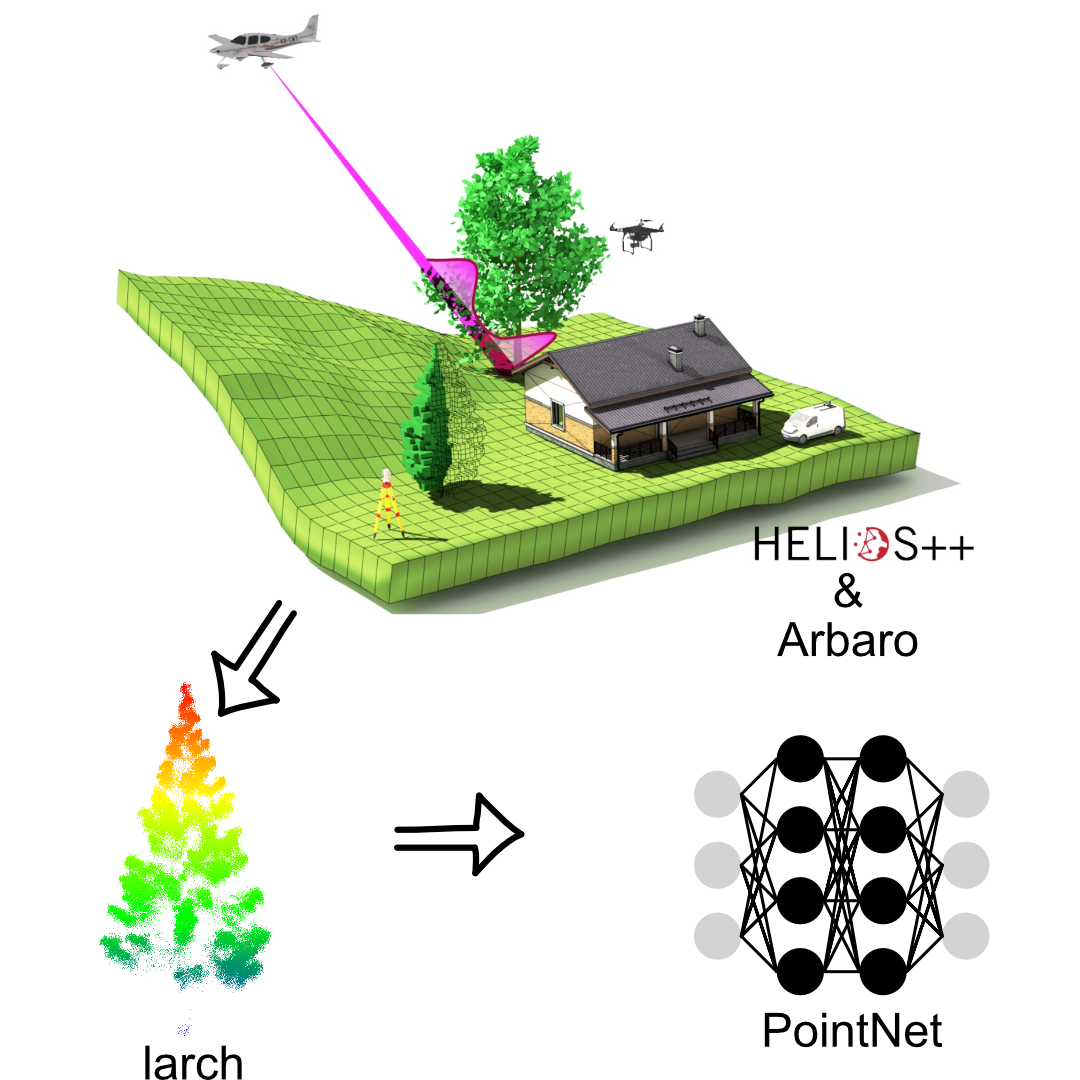
\includegraphics[width=\textwidth]{assets/workflow_synthetic_data}
        \end{column}
    \end{columns}
\end{frame}

\section{Methods}
\sectionIntroHidden % Show an outline of the current section with hidden subsections
%\sectionIntro % Show an outline of the current section with subsections

\begin{frame}{Methods}

    \begin{itemize}
        \item data loading
        \item trainin time
    \end{itemize}

\end{frame}


\section{Tools}

\begin{frame}{Tools - Overview}

% Please add the following required packages to your document preamble:
% \usepackage{booktabs}
\begin{table}[]
\begin{tabular}{@{}ll@{}}
\toprule
tool               & purpose \\ \midrule
tensorboard        &         \\
Vtune              &         \\
likwid             &         \\
PyTorch - built-in &         \\ \bottomrule
\end{tabular}
\end{table}

\end{frame}

\begin{frame}{Benchmarking is the first step of optimizing}
\label{pg:lastpage} % Label on last frame to get the page number for footer

\begin{columns}
        \begin{column}{0.5\textwidth}
            \centering
            \vspace{-1em}
            \begin{figure}
            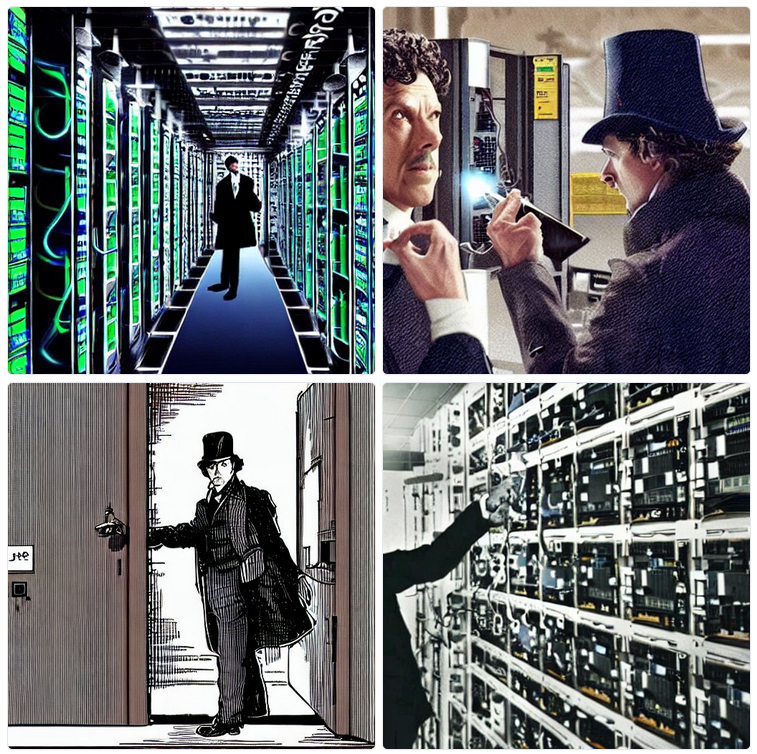
\includegraphics[width=0.85\textwidth]{assets/Sherlock-Holmes-locates-the-best-graphical-processing-unit-inside-the-data-center-for-his-deep-learning-workflow}
            \caption*{Image generated with stable diffusion: \\
            \tiny{"Sherlock Holmes locates the best graphical processing unit inside the data center for his deep learning workflow"}}
            \end{figure}
        \end{column}
        \begin{column}{0.5\textwidth}
            \begin{itemize}
                \item "Stable Diffusion v1 version of the model requires 150,000 A100 GPU Hours for a single training" session\footnote{\tiny{\url{https://syncedreview.com/2022/11/09/almost-7x-cheaper-colossal-ais-open-source-solution-accelerates-aigc-at-a-low-cost-diffusion-pretraining-and-hardware-fine-tuning-can-be/}}, Accessed on: 10.11.2022}
            \end{itemize}
        \end{column}
    \end{columns}

\end{frame}

\begin{frame}{References}
    % References slide in appendix
    \renewcommand*{\bibfont}{\normalfont\scriptsize}
    \printbibliography[heading=none]
\end{frame}

\end{document}
